% Numerical results (experiments E1--E3). Tables and figures are generated from saved results by
% experiments/tables.py and experiments/figures.py; no number in a table or figure is typed by hand.
\section{Numerical results}\label{sec:results}

The experiments verify the theoretical results of Sections~\ref{sec:setting}--\ref{sec:failure}.
All certificates use the S1-optimised multiplier with $\mX=\mK$, so $\alpha_X=s=1$. Three experiments are considered: E1 evaluates certificate
effectivity on two finite element benchmarks, E2 examines the restricted-support certificate floor, and E3 tests the theoretical properties on
random constrained quadratic problems. Results are pooled over three random seeds, $0$, $1$, and $2$.

\subsection{Benchmarks and corrections}\label{sec:setup}
\begin{table}[t]
\centering\small
\caption{The finite element benchmarks (read from the benchmark definitions and the settings of the code base).}
\label{tab:benchmarks}
% generated by experiments/tables.py; seeds [0, 1, 2]
\begin{tabular}{lll}
\hline
 & membrane & block \\
\hline
element & Quad4, scalar Laplace (2D) & Hex8, linear elasticity (3D) \\
mesh & $25\times25$ cells & $12\times12\times3$ cells \\
unknowns $N$ & 576 & 1452 \\
contact rows $n_c$ & 144 & 121 \\
training snapshots & 200 & 100 \\
test queries per seed & 200 & 100 \\
primal basis sizes $r$ & 5, 10, 20, 40, 60 & 4, 8, 15, 30 \\
\hline
\end{tabular}

\end{table}

Two finite element benchmarks are considered: a parametrised membrane and an elastic block, both employing constant stiffness matrices, node-selection contact constraints, and parameter-dependent loads and obstacles. The membrane uses $200$ training snapshots, $200$ test parameters per seed, and primal basis dimensions $r\in\{5,10,20,40,60\}$. The block uses $100$ training snapshots, $100$ test parameters per seed, and $r\in\{4,8,15,30\}$. Dual bases are constructed using nonnegative matrix factorisation. Across three random seeds, the experiments comprise $3{,}000$ membrane and $1{,}200$ block queries. The benchmark configurations are summarised in Table~\ref{tab:benchmarks}. All computations are carried out in double-precision floating-point arithmetic.

Three corrections defined in Section~\ref{sec:application} are considered: R0 (feasibility repair), R0s with gap-based snapping, and R0s with
multiplier-based snapping. Since test parameters are reused across basis dimensions and seeds, the queries are not statistically independent. The
reported percentages therefore describe the tested configurations rather than general certification probabilities. All correction parameters were
fixed before the experiments.

\subsection{E1: exactness and effectivity on finite element queries}\label{sec:e1}
\Cref{cor:exact} guarantees exact certification when $0\le\gh\le2\vg$ componentwise, denoted by condition (C). Otherwise, certificate
effectivity is bounded by Theorem~\ref{thm:missed}. Full-order solutions are computed for each query to evaluate the error, contact gaps, and
multipliers.

\begin{table}[t]
\centering\small
\caption{E1. Effectivity $\mathrm{eff}=\Dstar/\normK{\ve}$ with $\mX=\mK$. ``(C) holds'' is the share of queries with
$0\le\gh\le2\vg$; the column ``max$|\mathrm{eff}-1|$'' is restricted to these queries. ``Violations'' counts queries that
break the exactness (tolerance $10^{-6}$) or the bound of Theorem~\ref{thm:missed} (relative tolerance $10^{-9}$).}
\label{tab:e1}
\resizebox{\linewidth}{!}{% generated by experiments/tables.py; seeds [0, 1, 2]
\begin{tabular}{llrrrrrr}
\hline
problem & correction & queries & (C) holds & $\max|\mathrm{eff}-1|$ under (C) & median eff.\ otherwise & max eff.\ otherwise & violations \\
\hline
membrane & R0 & 3000 & 0\,\% & -- & 1.45 & 4.89 & 0 \\
membrane & R0s (gap rule) & 3000 & 40\,\% & 2.5e-14 & 1.09 & 1.87 & 0 \\
membrane & R0s (multiplier rule) & 3000 & 35\,\% & 2.7e-15 & 1.03 & 1.88 & 0 \\
block & R0 & 1200 & 8\,\% & 2.9e-14 & 1.50 & 3.15 & 0 \\
block & R0s (gap rule) & 1200 & 45\,\% & 3.0e-14 & 1.08 & 2.22 & 0 \\
block & R0s (multiplier rule) & 1200 & 71\,\% & 2.9e-14 & 1.01 & 1.35 & 0 \\
\hline
\end{tabular}
}
\end{table}

\begin{figure}[t]
\centering
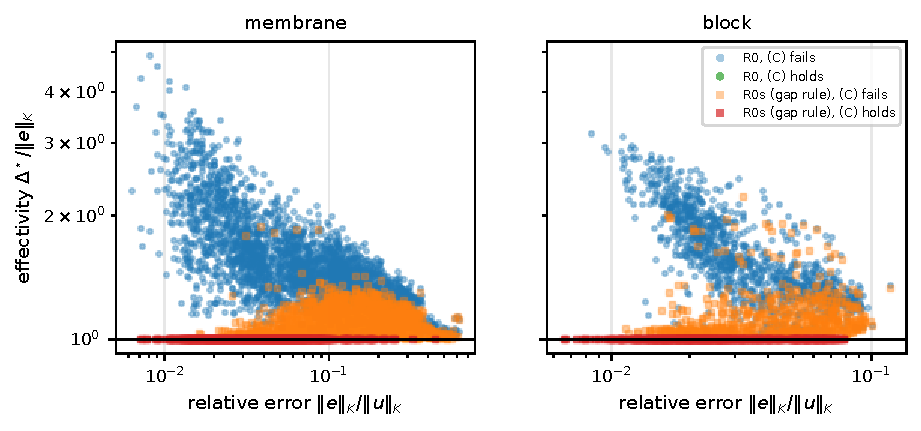
\includegraphics[width=\linewidth]{figures/fig_e1_effectivity}
\caption{E1. Effectivity against the relative energy error for R0 and R0s (gap rule). Points satisfying condition (C) lie on
$\mathrm{eff}=1$ (Corollary~\ref{cor:exact}); R0 does not satisfy (C) on the membrane. The figure illustrates the relation between condition (C) and the observed effectivity; it does not establish a convergence rate for approximations that violate (C).}
\label{fig:e1}
\end{figure}

\Cref{tab:e1} and \Cref{fig:e1} confirm that condition (C) yields unit effectivity to numerical precision. Its occurrence depends on the correction
method and benchmark. For the membrane, R0 never satisfies (C), whereas gap-based and multiplier-based snapping achieve $40\,\%$ and $35\,\%$,
respectively. For the block, the corresponding proportions are $8\,\%$, $45\,\%$, and $71\,\%$. When (C) is not satisfied, median effectivities
range from $1.01$ to $1.50$, with a maximum of $4.89$. All queries satisfy Theorem~\ref{thm:missed}, although the tightness of its bound and the
role of missed constraints in the largest effectivities remain unverified. Multiplier-based snapping achieves the highest exactness proportion on the
block but may reduce displacement accuracy through excessive snapping.

\subsection{E2: the support floor}\label{sec:e2}
Theorem~\ref{thm:support} establishes a positive asymptotic certificate floor when the multiplier support omits a strictly active constraint. This
is examined using predictions $\vu+\varepsilon\boldsymbol\varphi$, where $\boldsymbol\varphi=\mK^{-1}\mB\T\vlam$ is scaled so that
$\normK{\boldsymbol\varphi}=\normK{\vu}$, with $\varepsilon\in[10^{-6},10^{-1}]$. After correction on the exact strictly active set, each
approximation is certified using unrestricted S1 and two restricted supports: all rows except the largest-force active row $i^\ast$, and
$\Aplus\setminus\{i^\ast\}$. The floor $\sigma_S$ is computed offline using the exact multiplier. This controlled sequence tests the theoretical
result rather than representing typical reduced-order errors.

\begin{table}[t]
\centering\small
\caption{E2. At the smallest amplitude, the minimum over queries of the restricted certificate divided by the floor
$\sigma_S$ and by the full-S1 certificate; slope of the full-S1 certificate in the error (log--log). ``Violations'' counts
queries with ratio to $\sigma_S$ below $0.95$ or ratio to full S1 below $100$.}
\label{tab:e2}
\resizebox{\linewidth}{!}{% generated by experiments/tables.py; seeds [0, 1, 2]
\begin{tabular}{llrrrr}
\hline
problem & support $S$ & rate of full S1 & $\min\Delta^\star(\ell_S)/\sigma_S$ & $\min\Delta^\star(\ell_S)/\Delta^\star(\ell^\star)$ & violations \\
\hline
membrane & all rows but $i^\ast$ & 1.000 & 1.000 & 65044 & 0 \\
membrane & $\mathcal A_+\setminus\{i^\ast\}$ & 1.000 & 1.000 & 65044 & 0 \\
block & all rows but $i^\ast$ & 1.001 & 1.000 & 53449 & 0 \\
block & $\mathcal A_+\setminus\{i^\ast\}$ & 1.001 & 1.000 & 53449 & 0 \\
\hline
\end{tabular}
}
\end{table}

\begin{figure}[t]
\centering
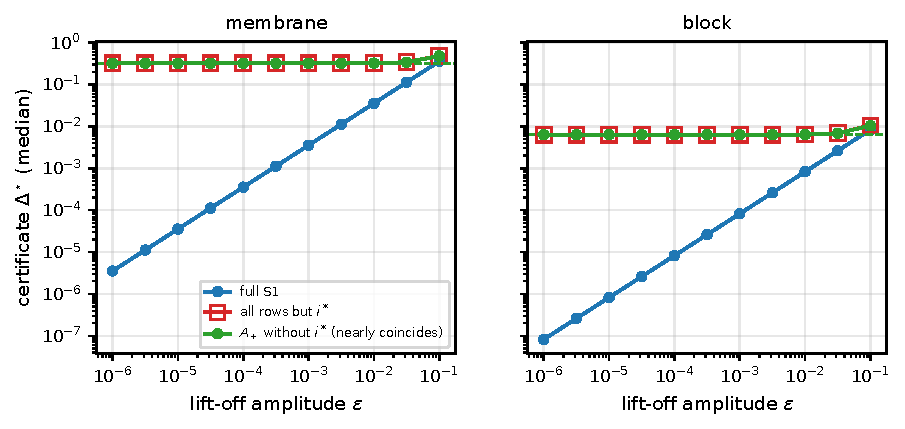
\includegraphics[width=\linewidth]{figures/fig_e2_support_floor}
\caption{E2. Median certificate against the amplitude $\varepsilon$ for full S1 and the two restricted supports (the two
restricted curves nearly coincide); dashed lines are the median floors $\sigma_S$, computed from the exact full-order multipliers for verification.}
\label{fig:e2}
\end{figure}

\Cref{tab:e2} and \Cref{fig:e2} show that unrestricted S1 converges linearly with the error, while both restricted certificates approach the predicted
floor. At the smallest amplitude, the restricted certificates exceed the unrestricted values by more than $5\times10^4$. The two supports produce
nearly identical certificate values, although their optimising multipliers differ (additional diagnostics are reported in
Appendix~\ref{app:e2diag}). This observed agreement is not asserted as a general identity. The result also holds for the block, whose correction
direction contains both positive and negative components and whose stiffness matrix is not an M-matrix.

\subsection{E3: property tests on random instances}\label{sec:e3}
The theoretical statements of Sections~\ref{sec:setting}--\ref{sec:failure} are tested on random constrained quadratic problems with full-row-rank
matrices $\mB$, symmetric positive-definite matrices $\mK$, and either $\mX=\mK$ or a random positive-definite $\mX$ with $s>1$. Four problem
sizes and five categories of feasible approximations are considered. Exact solutions are obtained from the condensed complementarity problem and
refined using equality-constrained KKT solves. Each of three seeds generates $1,000$ instances. No violations are observed under the specified
numerical tolerances (\Cref{tab:e3} in Appendix~\ref{app:e3}). The efficiency bound of Theorem~\ref{thm:efficiency} has a median ratio of
$0.87$ and a minimum of $0.34$, while Theorem~\ref{thm:missed} gives a median ratio of $0.71$. The lower bound of Theorem~\ref{thm:support}
is attained within $0.1\,\%$ in the most favourable instance. These tests verify algebraic consistency; contact-specific behaviour is examined
separately in E1 and E2.

\paragraph{Numerical verification adjustments.}
Four adjustments were made after the initial runs. First, the energy identity of Proposition~\ref{prop:gap} was evaluated in an algebraically
stable form to avoid cancellation, while direct energy differences were retained as diagnostics. Second, reference solutions were refined using
equality-constrained KKT solves. Third, rounding allowances proportional to $16\,n\,\varepsilon_{\rm mach}$ were introduced for the gap identity;
observed discrepancies remained within $2.4\,\%$ of these allowances. Finally, an unnecessary M-matrix check was removed from E2 because the
tested result does not require this property. All reported results use the revised verification procedures.
